\section{CTST - Lớp 10 - Ôn tập giữa học kì 1 - Đề 5}
\caulc
\Opensolutionfile{ans}[ans-ABCD]
%%%=============EX_1=============%%%
\begin{ex}%[0D1N1-2]
	Trong các mệnh đề sau, tìm mệnh đề đúng?
	\choice
	{$\pi < 2$}
	{$\pi^2> 16$}
	{$\sqrt{23} > 5$}
	{\True $\sqrt{25} \geq 5$}
	\loigiai{
		Ta có $\sqrt{25} \geq 5$ nên $\sqrt{25} \geq 5$ là mệnh đề đúng.}
\end{ex}
%%%=============EX_2=============%%%
\begin{ex}%[0D1N1-2]
	Cho mệnh đề chứa biến $P(x)\colon$\lq\lq $x+15\leq x^2$\rq\rq\ với $x$ là số thực. Mệnh đề nào sau đây là đúng
	\choice
	{$P(0)$}
	{$P(3)$}
	{$P(4)$}
	{\True $P(6)$}
	\loigiai{Ta có $P(6)\colon$\lq\lq $6+15\leq 6^2$\rq\rq\ là mệnh đề đúng.}
\end{ex}
%%%=============EX_3=============%%%
\begin{ex}%0D1N3-1]
	Cho $A$, $B$ là hai tập hợp được minh họa như hình vẽ. Phần tô đen trong hình vẽ là tập hợp nào sau đây?
	\begin{center}
		\begin{tikzpicture}
			\def\miena{(0,0)to [bend left=90] (2,2) to[bend left=90] (0,0) }
			\def\mienb{(1,0)to [bend left=90] (3,2) to[bend left=90] (1,0) }
			\begin{scope}
				\clip \miena;
				\draw[pattern=north east lines] \mienb;
			\end{scope}
			\draw \miena \mienb;
			\draw (0.2,0.5)node[above]{$A$} (2.6,1.3)node[above]{$B$};
		\end{tikzpicture}
	\end{center}
	\choice
	{\True $A\cap B$}
	{$A\cup B$}
	{$A\setminus B$}
	{$B\setminus A$}
	\loigiai{Dựa vào hình vẽ ta thấy phần tô đen là $A\cap B$.}
\end{ex}
%%%=============EX_4=============%%%
\begin{ex}%[0D1N2-1]
	Cho tập hợp $B$ gồm các số tự nhiên có một chữ số và chia hết cho $3$. Khi đó tập hợp $B$ viết theo cách liệt kê các phần tử của tập hợp là
	\choice
	{$B=\{3; 6; 9; 12\}$}
	{\True $B=\{0; 3; 6; 9\}$}
	{$B=\{n \in \mathbb{N}\mid 0\leq n \leq 9$ và $n \vdots 3\}$}
	{$B=\{n \in \mathbb{N}\mid 0< n \leq 9$ và $n: 3\}$}
	\loigiai{
		Tập hợp $B$ gồm các số tự nhiên có một chữ số và chia hết cho $3$ được viết theo cách liệt kê các phần tử của tập hợp là $B=\{0; 3; 6; 9\}$.}
\end{ex}
%%%=============EX_5=============%%%
\begin{ex}%[0D2N1-1]
	Cặp số nào sau đây không là nghiệm của bất phương trình $2x+y-7> 0$.
	\choice
	{$(3; 2)$}
	{$(5;-1)$}
	{$(4; 0)$}
	{\True $(-2; 5)$}
	\loigiai{Thay lần lượt các cặp số $(x; y)$ ở trong đáp án vào bất phương trình $2x+y-7> 0$, chỉ có cặp $(-2; 5)$ không thỏa mãn.}
\end{ex}
%%%=============EX_6=============%%%
\begin{ex}%0D3N1-2]
	Tập xác định của hàm số $f(x)=\dfrac{3x-6}{4x-12}$ là
	\choice
	{$\mathscr{D}=\mathbb{R}$}
	{$\mathscr{D}=(3;+\infty)$}
	{$\mathscr{D}=\mathbb{R} \setminus\{2\}$}
	{\True $\mathscr{D}=\mathbb{R} \setminus\{3\}$}
	\loigiai{
		Biểu thức $\dfrac{3x-6}{4x-12}$ có nghĩa khi $4x-12\neq 0\Leftrightarrow x \neq 3$.\\
		Vậy tập xác định của hàm số đã cho là $\mathscr{D}=\mathbb{R} \setminus\{3\}$.}
\end{ex}
%%%=============EX_7=============%%%
\begin{ex}%[0D3H2-2]
	Hàm số $y=2x^2+4x-2023$
	\choice
	{Đồng biến trên khoảng $(-\infty;-2)$ và nghịch biến trên khoảng $(-2;+\infty)$}
	{Nghịch biến trên khoảng $(-\infty;-2)$ và đồng biến trên khoảng $(-2;+\infty)$}
	{Đồng biến trên khoảng $(-\infty;-1)$ và nghịch biến trên khoảng $(-1;+\infty)$}
	{\True Nghịch biến trên khoảng $(-\infty;-1)$ và đồng biến trên khoảng $(-1;+\infty)$}
	\loigiai{
		Hàm số $y=a x^2+b x+c$ với $a > 0$ đồng biến trên khoảng $\left(-\dfrac{b}{2a};+\infty\right)$, nghịch biến trên khoản $\left(-\infty;-\dfrac{b}{2a}\right)$.\\
		Áp dụng: ta có $-\dfrac{b}{2a}=-1$.\\
		Do đó hàm số nghịch biến trên khoảng $(-\infty;-1)$ và đồng biến trên khoảng $(-1;+\infty)$.}
\end{ex}
%%%=============EX_8=============%%%
\begin{ex}%[0D3H2-3]
	\immini{Hàm số nào có đồ thị như hình vẽ bên?
		\choice
		{\True $y=-x^2+4x-3$}
		{$y=-x^2-4x-3$}
		{$y=-2x^2-x-3$}
		{$y=x^2-4x-3$}}{
		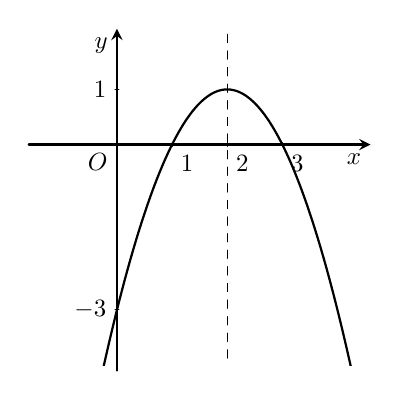
\begin{tikzpicture}[line join=round, line cap=round,>=stealth,thick,scale=.7]
			\tikzset{every node/.style={scale=0.9}}
			\draw[->] (-1.6,0)--(4.6,0) node[below left] {$x$};
			\draw[->] (0,-4.1)--(0,2.1) node[below left] {$y$};
			\draw (0,0) node [below left] {$O$};
			\foreach \x/\nx in {1/1,2/2,3/3}
			\draw[thin] (\x,1pt)--(\x,-1pt) node [below right] {$\nx$};
			\foreach \y/\ny in {1/1,-3/-3}
			\draw[thin] (1pt,\y)--(-1pt,\y) node [left] {$\ny$};
			\begin{scope}
				\clip (-1.5,-4) rectangle (4.5,2);
				\draw[samples=200,domain=-0.3:4.3,smooth,variable=\x] plot (\x,{-1*(\x)^2+4*(\x)-3});
			\end{scope}
			\draw [dashed, thin] (2,2)--(2,-4);
	\end{tikzpicture}}
	\loigiai{
		Đồ thị có bề lõm quay xuống dưới nên $a < 0$. Loại phương án $y=x^2-4x-3$.\\
		Trục đối xứng $x=2$ và có tọa độ đỉnh $I(2;1)$.\\
		Vậy hàm số ứng đồ thị đã cho là $y=-x^2+4x-3$.}
\end{ex}
%%%=============EX_9=============%%%
\begin{ex}%[0H4H1-2]
	Cho $90^{\circ} < \alpha < 180^{\circ}$. Khẳng định nào sau đây đúng?
	\choice
	{$\cos \alpha > 0$}
	{\True $\sin \alpha > 0$}
	{$\tan \alpha > 0$}
	{$\cot \alpha > 0$}
	\loigiai{
		Vì $90^{\circ} < \alpha < 180^{\circ}$ nên $\sin \alpha > 0$, $\cos \alpha < 0$, $\tan \alpha < 0$, $\cot \alpha < 0$.}
\end{ex}
%%%=============EX_10=============%%%
\begin{ex}%[0H4H1-1]
	Cho $0^{\circ} < \alpha < 180^{\circ}$ và $\alpha \neq 90^{\circ}$. Khẳng định nào sau đây \textbf{sai}?
	\choice
	{\True $\sin \left(180^{\circ}-\alpha\right)=-\sin \alpha$}
	{$\cos \left(180^{\circ}-\alpha\right)=-\cos \alpha$}
	{$\tan \left(180^{\circ}-\alpha\right)=-\tan \alpha$}
	{$\cot \left(180^{\circ}-\alpha\right)=-\cot \alpha$}
	\loigiai{
		Ta có $\sin \left(180^{\circ}-\alpha\right)=\sin \alpha$.}
\end{ex}
%%%=============EX_11=============%%%
\begin{ex}%[0D2H1-1]
	Cặp số $(x; y)$ nào sau đây là một nghiệm của hệ bất phương trình $\heva{&2x-y \leq 0\\&x+3y-1> 0}$?
	\choice
	{$(x; y)=(-2;-1)$}
	{$(x; y)=(4; 0)$}
	{\True $(x; y)=(1; 2)$}
	{$(x; y)=(-3;-4)$}
	\loigiai{
		Thay $x=1$; $y=2$ vào hệ bất phương trình ta có $\heva{&2x-y=0\leq 0\\
			&x+3y-1=6> 0}$ thỏa mãn.\\
		Vậy $(x; y)=(1; 2)$ là một nghiệm của hệ bất phương trình.}
\end{ex}
%%%=============EX_12=============%%%
\begin{ex}%[0D3H2-2]
	Cho hàm số $y=-x^2+4x-3$. Khẳng định nào sau đây đúng?
	\choice
	{Hàm số nghịch biến trên khoảng $(-\infty; 2)$}
	{\True Hàm số đồng biến trên khoảng $(-\infty; 2)$}
	{Hàm số đồng biến trên khoảng $(3;+\infty)$}
	{Hàm số nghịch biến trên khoảng $(1; 3)$}
	\loigiai{
		Ta có tọa độ đỉnh $I(2; 1)$.\\
		Bảng biến thiên
		\begin{center}
			
\begin{tikzpicture}				\tkzTabInit[nocadre=true,lgt=1.2,espcl=2.5,deltacl=0.5]
				{$x$ /0.75, $y$/2}
				{$ -\infty $,$ 2 $,$ +\infty $}				\tkzTabVar{-/$-\infty$,+/$1$,-/$-\infty$} %+ hoac-
			\end{tikzpicture}
		\end{center}
		Vậy hàm số đồng biến trên khoảng $(-\infty; 2)$ và nghịch biến trên $(2;+\infty)$.
	}
\end{ex}
\Closesolutionfile{ans}
\indapan{6}{ans-ABCD}

\cauds
\Opensolutionfile{ans}[ans-DS]
\begin{ex}%[0D1V3-5]
	Lớp $10A$ có $36$ học sinh, trong đó có $20$ bạn thích bóng rổ, $14$ bạn thích bóng bàn và $10$ bạn không thích môn thể thao nào trong hai môn thể thao này. Các khẳng định sau đây đúng hay sai?
	\choiceTF
	{\True Số học sinh thích một trong hai môn thể thao là $26$}
	{\True Số học sinh thích cả hai môn thể thao là $8$}
	{\True Số học sinh thích bóng rổ nhưng không thích bóng bàn là $12$}
	{Số học sinh thích bóng bàn nhưng không thích bóng rổ là $10$}
	\loigiai{
		Gọi 
		\begin{itemize}
			\item $A$ là tập hợp các học sinh của lớp $10 A$;
			\item $B$ là tập hợp các bạn thích bóng rổ;
			\item $C$ là tập hợp các bạn thích bóng bàn;
			\item $D$ là tập hợp các bạn không thích môn nào trong hai môn.
		\end{itemize}
		Ta có $n(A)=36$, $n(B)=20$, $n(C)=14$, $n(D)=10$.
		\begin{itemchoice}
			\itemch \textbf{Đúng.}\\ 
			Số học sinh thích một trong hai môn thể thao là
			\[n(B \cup C)=n(A)-n(D)=36-10=26.\]
			\itemch \textbf{Đúng.}\\
			Số học sinh thích cả hai môn thể thao là
			\[n(B \cap C)=n(B)+n(C)-n(B \cup C)=20+14-26=8.\]
			\itemch \textbf{Đúng.}\\
			Số học sinh thích bóng rổ nhưng không thích bóng bàn là
			\[n(B \backslash C)=n(B)-n(B \cap C)=20-8=12.\]
			\itemch \textbf{Sai.}\\
			Số học sinh thích bóng bàn nhưng không thích bóng rổ là
			\[n(C \backslash B)=n(C)-n(B \cap C)=14-8=6.\]
	\end{itemchoice}}
\end{ex}

%%%==============EX_1============%%%
\begin{ex}%[0D2V2-2] 
	Cho hệ bất phương trình $\heva{&3x+2y \geq 9\\&x-2y \leq 3\\&x+y \leq 6\\	&x \geq 1} \quad(I)$.\\
	Các khẳng định sau là đúng hay sai?
	\choiceTF
	{$(1;-1)$ là nghiệm của bất phương trình $3x+2y \geq 9$}
	{\True $(3; 2)$ là một nghiệm của hệ bất phương trình $(I)$}
	{\True Miền nghiệm của hệ bất phương trình là miền tam giác}
	{Với $(x; y)$ thuộc miền nghiệm của hệ $(I)$, biểu thức $F=3x-y$ đạt giá trị lớn nhất bằng $14$}
	\loigiai{
		\begin{itemchoice}
			\itemch \textbf{Sai.}\\
			Thay $x=1$, $y=-1$ vào bất phương trình $3x+2y \geq 9$.\\
			Ta được \[3\cdot 1+2\cdot (-1) \geq 9\,text{(Sai).}\]		
			Vậy $(1;-1)$ không là nghiệm của bất phương trình $3x+2y \geq 9$.
			\itemch \textbf{Đúng.}\\
			Thay $x=3$, $y=2$ vào hệ bất phương trình $(I)$ ta có $\heva{&3\cdot 3+2\cdot 2\geq 9\\&3-2\cdot 2\leq 3\\&3+2\leq 6\\&3\geq 1&}$ (Đúng).\\			
			Vậy $(3;2)$ là nghiệm của hệ bất phương trình $(I)$.
			\itemch \textbf{Sai.}\\
			\immini{Miền nghiệm của hệ $(I)$ là miền trong của tứ giác $ABCD$ kể cả bờ là các đoạn thẳng $AB$, $BC, CD, AD$ với $A(3; 0)$, $B(5; 1)$, $C(1; 5)$, $D(1; 3)$ (miền không bị gạch bỏ ở hình vẽ bên).}
			{\begin{tikzpicture}[scale=0.7, line join=round, line cap=round, >=stealth]
					\tikzset{every node/.style={scale=1}}
					\def\xmin{-3}\def\xmax{7}\def\ymin{-3}\def\ymax{8}
					\draw[->] (\xmin-0.2,0)--(\xmax+0.2,0) node[below]{$x$};
					\draw[->] (0,\ymin-0.2)--(0,\ymax+0.2) node[right]{$y$};
					\draw (0,0) node[below left]{$O$};
					\foreach \x in {1,3,5,6}\draw (\x,0.1)--(\x,-0.1) node[below]{$\x$};
					\foreach \y in {1,3,5,6}\draw (0.1,\y)--(-0.1,\y) node[above left]{$\y$};
					\clip (\xmin,\ymin) rectangle (\xmax,\ymax);
					
					\draw[thick,smooth,samples=200,domain=\xmin:\xmax] plot (\x,{(-3/2)*(\x)+(9/2)});
					\clip (\xmin,\ymin) rectangle (\xmax,\ymax);
					
					\draw[thick,smooth,samples=200,domain=\xmin:\xmax] plot (\x,{(1/2)*(\x)-(3/2)});
					
					\draw[thick,smooth,samples=200,domain=\xmin:\xmax] plot (\x,{-1*(\x)+6});
					
					\draw[thick,smooth,samples=200,domain=\xmin:\xmax] (1,-3) -- (1,8);
					
					\fill[pattern=north east lines,smooth]
					plot[domain=-3:7] (\x,{(-3/2)*(\x)+(9/2)})
					-- plot[domain=7:-3] (\x,{0*(\x)-5})
					-- cycle;
					
					\fill[pattern=north east lines,smooth]
					plot[domain=-3:7] (\x,{(1/2)*(\x)-(3/2)})
					-- plot[domain=7:-3] (\x,{0*(\x)-5})
					-- cycle;
					
					\fill[pattern=north east lines,smooth]
					plot[domain=-3:7] (\x,{0*(\x)+8})
					-- plot[domain=7:-3] (\x,{-1*(\x)+6})
					-- cycle;
					
					\fill[pattern=north east lines,smooth]
					plot[domain=-3:1] (\x,{0*(\x)+8})
					-- plot[domain=1:-3] (\x,{0*(\x)-3})
					-- cycle;
					
					\path
					(3,0) node[above]{$A$}
					(5,1) node[above]{$B$}
					(1,5) node[above right]{$C$}
					(1,3) node[above right]{$D$}
					;
			\end{tikzpicture}}
			\itemch \textbf{Đúng.}\\
			Tính giá trị của $F=3x-y$ tại các cặp số $(x; y)$ là toạ độ của các đỉnh tứ giác $ABCD$, ta có
			\begin{itemize}
				\item Tại điểm $A(3; 0)$: $F=3\cdot 3-0=9$;
				\item Tại điểm $B(5; 1)$: $F=3\cdot 5-1=14$;
				\item Tại điểm $C(1; 5)$: $F=3\cdot 1-5=-2$;
				\item Tại điểm $D(1; 3)$: $F=3\cdot 1-3=0$.
			\end{itemize}
			Vậy $F$ đạt giá trị lớn nhất bằng $14$ tại $x=5, y=1$.
		\end{itemchoice}
	}
\end{ex}
%%%==============EX_2============%%%
\begin{ex}%[0D3V1-4] 
	Cho hàm số $y=f(x)$ có đồ thị như hình vẽ.
	\begin{center}
		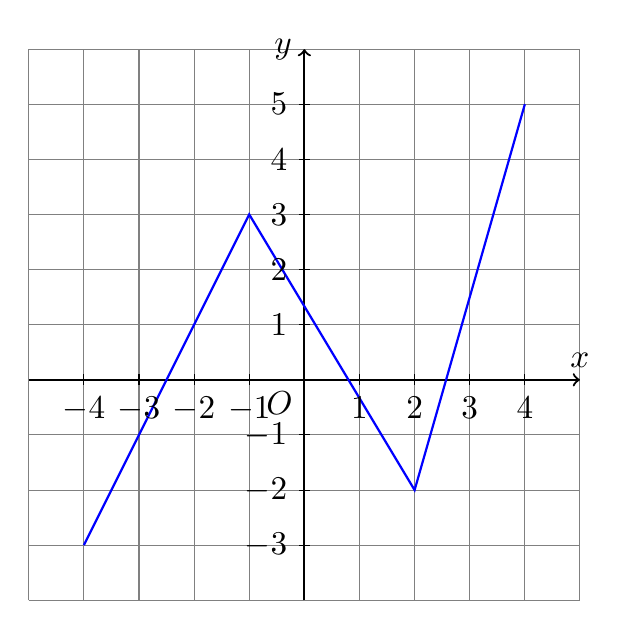
\begin{tikzpicture}[scale=0.7]
			\draw[step=1,gray,thin] (-5,-4) grid (5,6);
			\draw[->,thick](-5,0)--(5,0) node[above]{$x$};
			\draw[->,thick](0,-4)--(0,6) node[left]{$y$};
			\draw[blue,thick] (-4,-3)--(-1,3)--(2,-2)--(4,5);
			\draw (0,0) node[below left]{$O$};
			\foreach \x in {-4,-3,-2,-1,1,2,3,4} \draw (\x,0.1)--(\x,-0.1) node[below]{$\x$};
			\foreach \y in {-3,-2,-1,1,2,3,4,5}\draw (0.1,\y)--(-0.1,\y) node[left]{$\y$};		
		\end{tikzpicture}
	\end{center}
	\choiceTF
	{\True Tập xác định của hàm số $y=f(x)$ là $\mathscr{D}=[-4; 4]$}
	{Giá trị nhỏ nhất của hàm số $y=f(x)$ trên đoạn $[-1; 2]$ bằng $2$}
	{\True Điểm $M$ nằm trên đồ thị hàm số $y=f(x)$ có hoành độ $x_0\in[-4;-1]$ thì tung độ là $y_0=2x_0+5$}
	{Có duy nhất một giá trị nguyên dương của tham số $m$ để phương trình $2f(x)+1-m^2=0$ có hai nghiệm phân biệt}
	\loigiai{ 
		\begin{itemize}
			\item \textbf{Đúng.}\\
			Tập xác định của hàm số $y=f(x)$ là $\mathscr{D}=[-4; 4]$.
			\item \textbf{Sai.}\\
			Vì hàm số $y=f(x)$ nghịch biến trên đoạn $[-1; 2]$ nên giá trị nhỏ nhất của hàm số trên $[-1; 2]$ là $f(2)=-2\neq 2$.
			\item \textbf{Đúng.}\\
			Trên đoạn $[-4;-1]$ đồ thị hàm số $y=f(x)$ là đường thẳng đi qua hai điểm $(-4;-3)$ và $(-1; 3)$ nên có công thức xác định là $y=f(x)=2x+5$.\\
			Do đó, điểm $M$ nằm trên đồ thị hàm số $y=f(x)$ có hoành độ $x_0\in[-4;-1]$ thì tung độ là $y_0=2x_0+5$.
			\item \textbf{Sai.}\\
			Ta có
			\[2f(x)-1+m^2=0 \Leftrightarrow f(x)=\dfrac{1-m^2}{2}.\]
			Số nghiệm của phương trình $f(x)=\dfrac{1-m^2}{2}$ bằng số giao điểm của đồ thị hàm số với đường thẳng $y=\dfrac{1-m^2}{2}$ (song song hoặc trùng với trục hoành).\\
			Để phương trình $f(x)=\dfrac{1-m^2}{2}$ có hai nghiệm phân biệt khi và chỉ khi đường thẳng $y=\dfrac{1-m^2}{2}$ cắt đồ thị hàm số tại hai điểm phân biệt khi và chỉ khi
			\[
			\hoac{&\dfrac{1-m^2}{2}=-2\\&\dfrac{1-m^2}{2}=3} \Leftrightarrow\hoac{&m^2=5\\&m^2=-5\,\text{(vô nghiệm)}} \Leftrightarrow m=\pm \sqrt{5} \notin \mathbb{Z}^{+}.
			\]
		\end{itemize}
	}
\end{ex}
%%==============EX_3============%%%
\begin{ex}%[0D3V2-4] 
	Cho hàm số bậc hai $y=f(x)=x^2-3x+2$ có đồ thị $(P)$ là một parabol. Các khẳng định sau là đúng hay sai?
	\choiceTF
	{\True Parabol $(P)$ có bề lõm quay lên}
	{Trục đối xứng là đường thẳng có phương trình $y=\dfrac{3}{2}$}
	{\True Parabol $(P)$ cắt trục hoành tại hai điểm là $(1; 0)$ và $(2; 0)$}
	{Có hai giá trị nguyên của tham số $m$ để đường thẳng $(d)\colon y=(2m-1) x-m^2-m+3$ cắt $(P)$ tại hai điểm phân biệt có hoành độ $x_1; x_2$ thỏa mãn $\dfrac{1}{x_1}+\dfrac{1}{x_2}=4$}
	\loigiai{
		\begin{itemize}
			\item \textbf{Đúng.}\\ Vì parabol $(P)$ có hệ số $a=1 > 0$ nên nó có bề lõm quay lên.
			\item \textbf{Sai.}\\ Trục đối xứng là đường thẳng có phương trình $x=-\dfrac{b}{2a} \Leftrightarrow x=\dfrac{3}{2}$.
			\item \textbf{Đúng.}\\ Xét phương trình:
			\[
			f(x)=0 \Leftrightarrow x^2-3x+2=0 \Leftrightarrow \hoac{&x=1\\ &x=2.}
			\]
			Vậy parabol $(P)$ cắt trục hoành tại hai điểm là $(1; 0)$ và $(2; 0)$.
			\item \textbf{Sai.}\\ Xét phương trình hoành độ giao điểm của $(P)$ và $(d)$
			\[
			x^2-3x+2=(2m-1) x-m^2-m+3 \Leftrightarrow x^2-2(m+1) x+m^2+m-1=0 \quad (*)
			\]
			Ta có $\Delta^{\prime}=(m+1)^2-\left(m^2+m-1\right)=m^2+2m+1-m^2-m+1=m+2$.\\
			Để $(P)$ cắt $(d)$ tại hai điểm phân biệt có hoành độ khác 0, phương trình (*) phải có hai nghiệm phân biệt khác 0 khi và chỉ khi:
			\[
			\heva{&\Delta^{\prime} > 0\\ &c \neq 0} \Leftrightarrow \heva{&m > -2\\ &m^2+m-1 \neq 0.}
			\]
			Theo hệ thức Vi-et, ta có $
			\heva{&x_1+x_2=2(m+1)\\ &x_1x_2=m^2+m-1.}$
			Do đó
			\[
			\dfrac{1}{x_1}+\dfrac{1}{x_2}=4 \Leftrightarrow \dfrac{x_1+x_2}{x_1x_2}=4 \Leftrightarrow x_1+x_2=4x_1x_2.
			\]
			Thay vào ta được
			\[
			2(m+1)=4\left(m^2+m-1\right) \Leftrightarrow 4m^2+2m-6=0 \Leftrightarrow \hoac{&m=1\\ &m=-\dfrac{3}{2}.}\]
			Vậy chỉ có một giá trị nguyên của tham số $m$ thỏa mãn, đó là $m=1$.
		\end{itemize}
	}
\end{ex}
\Closesolutionfile{ans}

\indapan{3}{ans-DS}

\caukq

\Opensolutionfile{ans}[ans-KQ]

\begin{ex}%[0D1H2-3]
	Cho tập hợp $A=[m;m+2]$; $B=[-1;2)$ với $m$ là tham số. Có bao nhiêu giá trị nguyên $m$ để $A\subset B$.
	\shortans{$-1$}
	\loigiai{
		Ta có
		$A\subset B\Leftrightarrow\heva{&m\geq-1\\&m+2<2}\Leftrightarrow\heva{&m\geq-1\\&m<0}\Leftrightarrow-1\leq m<0$.\\
		Vậy $m=-1$
	}
\end{ex}

\begin{ex}%[0D2V2-3]
	Một công ty $X$ trong một đợt hỗ trợ xây dựng nông thôn mới cần thuê xe để chở ít nhất $120$ người và $6{,}5$ tấn hàng. Nơi thuê xe có hai loại xe $A$ và $B$, trong đó loại xe A có $9$ chiếc và loại xe $B$ có $8$ chiếc. Một chiếc xe loại A cho thuê với giá $4$ triêu đồng, một chiếc xe loại $B$ cho thuê với giá $3$ triệu đồng. Biết rằng mỗi chiếc xe loại A có thể chở tối đa $20$ người và $0{,}5$ tấn hàng; mỗi chiếc xe loại $B$ có thể chở tối đa $10$ người và $2$ tấn hàng. Hỏi chi phí thuê xe thấp nhất là bao nhiêu?
	\shortans{$26$}
	\loigiai{
		Gọi $x$ và $y$ lần lượt là số xe loại A và B mà công ty X đã thuê.\\
		Điều kiện $0\leq x\leq 9$; $x\in\mathbb{N}$ và $0\leq y\leq 8$; $y\in\mathbb{N}$.\\
		Số tiền cần bỏ ra để thuê xe là $f(x;y)=4x+3y$ (triệu đồng).\\
		Theo đề bài, ta có hệ bất phương trình
		$\heva{&0\leq x\leq 9\\&0\leq y\leq 8\\&20x+10y\geq 120\\&0,5x+2y\geq 6,5}\Leftrightarrow\heva{&0\leq x\leq 9\\&0\leq y\leq 8\\&2x+y\geq 12\\&x+4y\geq 13.}$\\
		Miền nghiệm của hệ bất phương trình trên là tứ giác $ABCD$ (kể cả biên) với $A(5;2)$; $B(9;1)$; $C(9;8)D(2;8)$ như hình vẽ.
		\begin{center}
			\begin{tikzpicture}[>=stealth,line join=round,line cap=round,scale=0.5 ,
				declare function={
					xmin=-1;
					xmax=10;
					ymin=-1;
					ymax=10;
					a=3;
					b=5;
					c=-5;
					f(\x)=-2*(\x)+12;
					g(\x)=-1*(\x)/4+3.25;
					quay=-45;
				} ]
				
				\begin{scope}
					\clip (xmin,ymin) rectangle (xmax,ymax);
					\fill [pattern=north east lines,pattern color=cyan ](xmax,-5)--(xmin,-5)--plot[domain=xmin:xmax](\x,{f(\x)})--cycle;
					\fill [pattern=north west  lines,pattern color=blue ](xmax,-5)--(xmin,-5)--plot[domain=xmin:xmax](\x,{g(\x)})--cycle;
					\fill [pattern=north west  lines,pattern color=red ](xmax,13)--(xmin,13)--plot[domain=xmin:xmax](\x,8)--cycle;	
					\fill [pattern=north west  lines,pattern color=orange ](xmax,-5)--(xmax,13)--plot[domain=ymax:ymin](9,\x)--cycle;	
					\draw[line width=1pt,red!80!black ] (xmin,{f(xmin)})--(xmax,{f(xmax)});
					\draw[line width=1pt,red!80!black ] (xmin,{g(xmin)})--(xmax,{g(xmax)});
					\draw[line width=1pt,red!80!black ] (xmin,8)--(xmax,8);
					\draw[line width=1pt,red!80!black ] (9,ymin)--(9,ymax);
					
				\end{scope}
				\draw[-stealth,line width=1pt](xmin,0)--(xmax,0)node[right]{$x$};
				\draw[-stealth,line width=1pt](0,ymin)--(0,ymax)node[above left]{$y$};
				\draw[dashed] (5,0)--(5,2)--(0,2)
				(2,0)--(2,8)--(0,8) (0,1)--(9,1)
				;
				\path (0,0) node[below right]{$O$}
				(5,2) node[below left]{$A$}
				(9,1) node[above right]{$B$}
				(9,8) node[above right]{$C$}
				(2,8) node[above right]{$D$}
				(2,0) node[below]{$2$}
				(5,0) node[below]{$5$}
				(9,0) node[below left]{$9$}
				(0,1) node[left]{$1$}
				(0,2) node[left]{$2$}
				(0,8) node[below left]{$8$}
				;
			\end{tikzpicture}
		\end{center}
		Ta có $f(5;2)=26$; $f(9;1)=39$; $f(9$; $8)=60$; $f(2$; $8)=32$.\\
		Suy ra $f(x;y)$ nhỏ nhất khi $(x; y)=(5; 2)$.\\
		Vậy chi phí thuê xe thấp nhất là $26$ triệu.
	}
\end{ex}

\begin{ex}%[0D2V2-2]
	Tìm giá trị lớn nhất biểu thức $F(x;y)=x-y+2024$ với điều kiện $\heva{&2x-y\geq 2\\&x-2y\leq 2\\&x+y\leq 5\\&y\geq 0}$
	\shortans{$2\,027$}
	\loigiai{
		Vẽ các đường thẳng 
		$d_1\colon 2x-y=2\Leftrightarrow 2x-y-2=0$; $d_2\colon x-2y=2\Leftrightarrow x-2y-2=0$; $d_3\colon x+y=5\Leftrightarrow x+y-5=0$ trên cùng một hệ trục tọa độ.\\
		Miền nghiệm của hệ bất phương trình $(1)$ là miền tứ giác $ABCD$ (phần tô đậm trên hình vẽ).
		\begin{center}
			\begin{tikzpicture}[>=stealth,line join=round,line cap=round,scale=0.5 ,
				declare function={
					xmin=-2;
					xmax=12;
					ymin=-2;
					ymax=8;
					a=3;
					b=5;
					c=-5;
					f(\x)=-1*(\x)+5;
					g(\x)=1*(\x)/2-1;
					h(\x)=2*(\x)-2;
				} ]
				
				\begin{scope}
					\draw[gray!50] (xmin,ymin) grid (xmax,ymax);
					\clip (xmin,ymin) rectangle (xmax,ymax);
					\draw[line width=1pt,red!80!black ] (xmin,{f(xmin)})--(xmax,{f(xmax)});
					\draw[line width=1pt,red!80!black ] (xmin,{g(xmin)})--(xmax,{g(xmax)});
					\draw[line width=1pt,red!80!black ] (xmin,{h(xmin)})--(xmax,{h(xmax)});
				\end{scope}
				\draw[-stealth,line width=1pt](xmin,0)--(xmax,0)node[right]{$x$};
				\draw[-stealth,line width=1pt](0,ymin)--(0,ymax)node[above left]{$y$};
				\path (0,0) node[below left]{$O$}
				(1,0) coordinate (D) node[above left]{$D$}
				(2,0) coordinate (C) node[below]{$C$}
				(6,2) coordinate (T) node[right]{$d_3\colon x-2y-2=0$}
				(4,1) coordinate (B) node[above]{$B$}
				(4,6) coordinate (E) node[right]{$d_1\colon 2x-y-2=0$}
				(-2,7) coordinate (F)
				(7,-2) coordinate (M) node[right]{$d_2\colon x+y-5=0$}
				(intersection of B--F and D--E) coordinate (A) node[right]{$A$};
				\fill [pattern=north west  lines,pattern color=blue ](A)--(B)--(C)--(D)--cycle;
			\end{tikzpicture}
		\end{center}
		Trong đó
		\begin{itemize}
			\item $A=d_1\cap d_3$, tọa độ điểm $A$ là nghiệm của hệ $\heva{&2x-y=2\\&x+y=5}\Leftrightarrow\heva{&x=\dfrac{7}{3}\\&y=\dfrac{8}{3}}\Rightarrow A\left(\dfrac{7}{3};\dfrac{8}{3}\right)$.
			\item $B=d_2\cap d_3$, tọa độ điểm $B$ là nghiệm của hệ $\heva{&x-2y=2\\&x+y=5}\Leftrightarrow\heva{&x=4\\&y=1}\Rightarrow B(4;1)$.
			\item $C=d_2\cap Ox$, tọa độ điểm $C$ là nghiệm của hệ $\heva{&x-2y=2\\&y=0}\Leftrightarrow\heva{&x=2\\&y=0}\Rightarrow C(2;0)$.
			\item $D=d_1\cap Ox$, tọa độ điểm $D$ là nghiệm của hệ $\heva{&2x-y=2\\&y=0}\Leftrightarrow\heva{&x=1\\&y=0}\Rightarrow D(1;0)$.
		\end{itemize}
		
		\begin{itemize}
			\item Thay $x=\dfrac{7}{3}$; $y=\dfrac{8}{3}$ vào $F(x;y)=x-y+2\,024$ ta được $F\left(\dfrac{7}{3};\dfrac{8}{3}\right)=\dfrac{6\,071}{3}$.
			\item Thay $x=4; y=1$ vào $F(x;y)=x-y+2\,024$ ta được $F(4;1)=2\,027$.
			\item Thay $x=2; y=0$ vào $F(x;y)=x-y+2\,024$ ta được $F(2;0)=2\,026$.
			\item Thay $x=1; y=0$ vào $F(x;y)=x-y+2\,024$ ta được $F(1;0)=2\,025$.
		\end{itemize}
		Ta có $\dfrac{6\,071}{3}<2\,025<2\,026<2\,027$.\\
		Vậy giá trị lớn nhất biểu thức $F(x; y)=x-y+2\,024$ thỏa mãn điều kiện (I) là $2\,027$ tại $(4;1)$.
	}
\end{ex}

\begin{ex}%[0D2V2-3]
	Một công ty dịch vụ cho thuê xe hơi vào dịp tết với giá thuê mỗi chiếc xe hơi như sau: khách thuê tối thiểu phải thuê trọn ba ngày tết (mùng $1$, $2$, $3$) với giá $1\,000\,000$ đồng/ngày; những ngày còn lại (nếu khách còn thuê) sẽ được tính giá thuê là $700\,000$ đồng/ngày. Anh Việt định dành ra một khoản tối đa là $5\,500\,000$ đồng cho phí thuê xe đi chơi trong dịp tết. Hỏi anh Việt có thể thuê xe của công ty trên tối đa bao nhiêu ngày?
	\shortans{$6$}
	\loigiai{
		Ta có $T=3\,000\,000+700\,000\cdot(x-3)=900\,000+700\,000\cdot x$ với $x\geq 3$, $x\in\mathbb{N}$.\\
		Xét bất phương trình \[900\,000+700\,000\cdot x\leq 550\,0000\Leftrightarrow 9+7x\leq 55\Leftrightarrow x\leq\dfrac{46}{7}\approx 6{,}57.\]
		Vậy với khoản tiền $5\,500\,000$ đồng, anh Việt chỉ có thể thuê một chiếc xe của công ty tối đa $6$ ngày.
	}
\end{ex}

\begin{ex}%[0D3V2-6]
	Cổng Arch tại thành phố St Louis của Mỹ có hình dạng là một parabol (hình vẽ). Biết khoảng cách giữa hai chân cổng bằng $162$ m.Trên thành cổng, tại vị trí có độ cao $43$ m so với mặt đất (điểm $M$), người ta thả một sợi dây chạm đất (dây căng thẳng theo phương vuông góc với mặt đất). Vị trí chạm đất của đầu sợi dây này cách chân cổng A một đoạn $10$ m. Giả sử các số liệu trên chính xác. Hãy tính độ cao của cổng Arch (tính từ mặt đất đến điểm cao nhất của cổng, kết quả làm tròn đến hàng đơn vị).
	\begin{center}
		\begin{tikzpicture}[line join=round, line cap=round,>=stealth,thick]
			\tikzset{every node/.style={scale=1.2}}
			\draw[->] (-2,0)--(11,0) node[below left] {$x$};
			\draw[->] (0,-1)--(0,8) node[below left] {$y$};
			\draw (0,0) node [below left] {$O$};
			\begin{scope}
				\draw [red] (0,0).. controls +(0:0) and +(0:0) ..(1,2)
				.. controls +(0:0) and +(180:1.9) ..(5,6)
				.. controls +(0:1.9) and +(0:0) ..(9,2)
				.. controls +(0:0) and +(0:0) ..(10,0);
			\end{scope}
			\foreach \x/\y in {1/2,0/0,1/0,5/6}{
				\fill [blue] (\x,\y) circle (2pt);
			}
			\path
			(0,0) node[above left]{$A$}
			(1,2) node[above left]{$M$}
			(0.5,0) node[below]{$10m$}
			(1,1) node[right]{$43m$}
			(5,0) node[below]{$162m$}
			;
			\draw[dashed] (1,0)--(1,2)--(0,2);
		\end{tikzpicture}
	\end{center}
	\shortans{$186$}
	\loigiai{
		Chọn hệ trục tọa độ $Oxy$ như hình vẽ.\\
		Ta có $A(0;0)$; $B(162;0)$; $M(10;43)$.\\
		Giả sử phương trình của parabol $(P)$ là $y=ax^2+bx+c$.\\
		Do $A,B,M\in(P)$ nên toạ độ của chúng thỏa mãn phương trình $(P)$ ta có
		\[\heva{&a\cdot 162^2+b\cdot 162+c=0\\&a\cdot 10^2+b\cdot 10+c=43\\&c=0}\Leftrightarrow\heva{&a=-\dfrac{43}{1520}\\ &b=\dfrac{3483}{760}\\&c=0.}\]
		Suy ra $y=-\dfrac{43}{1520}x^2+\dfrac{3483}{760}x$.\\
		Chiều cao của cổng Arch là $h=-\dfrac{\Delta}{4a}\approx 186$ m. 
	}
\end{ex}

\begin{ex}%[0H4V1-3]
	Biết $2\sin^3a+\sin^2a-\sin^2a+5\sin a-3=0,(90^\circ < a < 180^\circ)$. Tính giá trị của biểu thức $P=\sqrt{3}\tan a-\sqrt{3}\cot(180^\circ-a)$.
	\shortans{$-4$}
	\loigiai{
		Ta có 
		\begin{eqnarray*}
			&&2\sin^3a+\sin^2a+5\sin a-3=0\\
			&\Leftrightarrow&\sin a=\dfrac{1}{2}\\
			&\Rightarrow&\cos a=-\dfrac{\sqrt{3}}{2}\; (\text{Vì\,}90^\circ<a<180^\circ)\\
			&\Rightarrow&\tan a=-\dfrac{1}{\sqrt{3}}\\
			&\Rightarrow&\cot a=-\sqrt{3}.
		\end{eqnarray*}
		Ta có $P=\sqrt{3}\tan a-\sqrt{3}\cot(180^\circ-a)=\sqrt{3}\cdot\dfrac{-1}{\sqrt{3}}-\sqrt{3}\cdot \sqrt{3}=-4$.
	}
\end{ex}

\Closesolutionfile{ans}

\indapan{6}{ans-KQ}